\documentclass[12pt]{book}
\usepackage{graphicx}
\usepackage{csquotes}
\usepackage{etoolbox}
\usepackage{setspace}
\usepackage{float}
\usepackage[table,xcdraw]{xcolor}
\usepackage{amsmath, amsthm, amssymb, amsfonts}
\usepackage[T1]{fontenc}
\usepackage[utf8]{inputenc}
\AtBeginEnvironment{displayquote}{\small \singlespacing}


\begin{document}
\chapter{Analysis}
In the first part of this chapter we introduce some some theoretical arguments useful in the analysis. Then we start considering a basic version of the model, trying to understand the basic concepts and ensure that everything works fine. Then we try to explain what are the consequences of a specific agent's behavior and analyzing some aspects of the entire model.   

\subsection{Update Evaluation}
Analyzing how people update their knowledge database, we can find an exponential law.\\
Let $B$ be the \textbf{agent's boldness}, $Q$ the \textbf{real quality} of a restaurant and $V$ the \textbf{internal valuation }about that restaurant. \\   
Thought by the agent on his own, people update $V$ step by step with the following recursion rule
\[V\left( {t + 1} \right) = V\left( t \right) + B\left( {Q - V\left( t \right)} \right)\]
by considering an infinitesimal time step $dt$ we can look at this relation as a partial derivative that we could integrate 
\[\frac{1}{B}\frac{{dV}}{{dt}} = Q - V\left( t \right)\]
In light of this we obtain both an homogeneous solution:
\[\begin{array}{l}
\frac{1}{B}\frac{{dV}}{{dt}} =  - V\left( t \right)\\
V\left( t \right) = V\left( 0 \right){e^{ - Bt}}
\end{array}\]	
And a particular one:
\[V\left( t \right) = Q\]
Thus, the complete solution of this partial differential equation will be the following
\[\boxed{V\left( t \right) = {V_0}{e^{-Bt}} + Q}\]


\subsection{Analyzing the global knowledge}
Let’s now analyze the model on what concerns the global knowledge related to all agents about restaurant’s quality. As mentioned before each restaurant is characterized by a particular ranking value which outlines its quality. Moreover, the ranking is actually a dual variable: there’s the Real ranking $Q$ unknown to customers and the personal thinking, for each person, of restaurant’s quality, $V$; this ranking is, thus, strictly related to the agent’s knowledge database.\\
Thus, we introduce for, each restaurant, an uncertainty factor $K_{re}$ which is defined as the variance of the evaluation of all the people at the specific time step $t$:

\begin{equation}
  {K_{re}}\left( t \right) = {\sum\limits_{per} {\left( {\mu \left( t \right) - {V_{re,per}}\left( t \right)} \right)} ^2}
\end{equation}
As a natural consequence, the global uncertainty $K$ is simply the mean value of $K_{re}$ estimated over all restaurants: 

\begin{equation}
  K\left( t \right) = \mathbb{E}\left[ {{K_{re}}\left( t \right)} \right]
\end{equation}



\section{First simulation: one restaurant}

In order to study how people update their thinking of each restaurant we start with a very simple situation: 1 restaurant, 20 persons and no friends. As  mathematically proved before, we can easily verify that every person updates his knowledge database following an exponential law.
It is important to outline that different people, with different boldness coefficient, will converge to the true restaurant quality in different ways. As we could expect people who are more obstinate (higher boldness) will be slower in converging to the true value of the restaurant; people more open-minded, instead, will be more incline in updating their knowledge database faster.
Computing the average valuation and the standard deviation over time

\begin{figure}[h!]
  \centering
  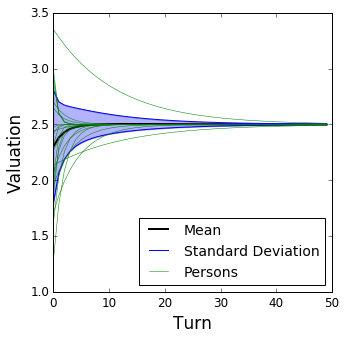
\includegraphics[width=7cm]{f1.png}
  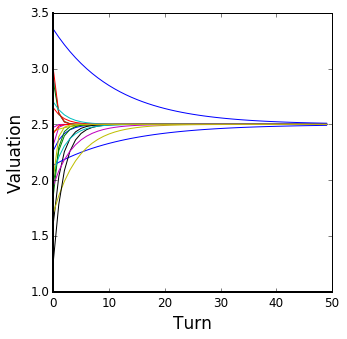
\includegraphics[width=6cm]{f2.png}
  \caption{Each color represents the personal thinking of a person. For the simulation we set 1 restaurant, 20 persons and no friends; the restaurant capaciter set high enough to host all people.}
  \label{fig:First simulation}
\end{figure}


Lead us to compute even $K_{re}$ coefficient. 
\begin{figure}[h!]
  \centering
  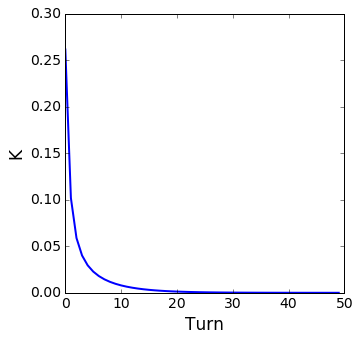
\includegraphics[width=7cm]{f3.png}
  \caption{Each color represents the personal thinking of a person. For the simulation we set 1 restaurant, 20 persons and no friends; the restaurant capaciter set high enough to host all people.}
  \label{fig:First simulation}
\end{figure}
As we see in plot \ref{fig:First simulation}, the $K_{re}$ coefficient after a sufficient number of turns converge to $0$, this means that at $t \to \infty$ all people will know the real quality of the restaurant $Q$.



\section{Second simulation: many restaurants}
In this second section we set up simulations by considering a more realistic situation with many restaurants. Since people now have to choose where to go among many places becomes important the waytough they take this choice. 

\subsubsection{Randomly choose}
People select randomly the place where to eat.
\begin{figure}[h!]
  \centering
  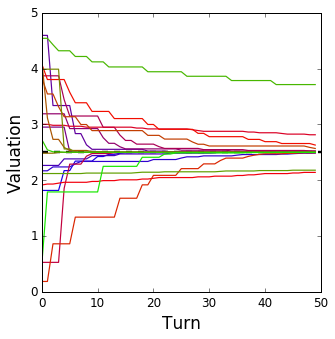
\includegraphics[width=7cm]{rand1.png}
  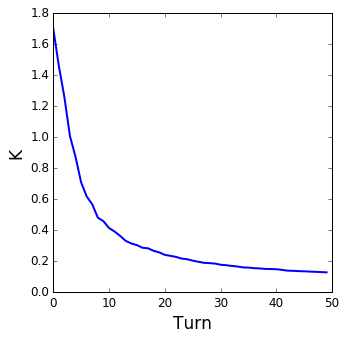
\includegraphics[width=6cm]{rand2.png}
  \caption{Simulation with:  4 restaurant, 20 persons, no friend, 50 turns, random choose.}
\end{figure}

In this case,  the process of updating the thinking is a bit different. Actually a person goes to different restaurants, and updates knowledge database only for that place; thus, since a person focuses only on a single restaurant we see that the curve is not an exponential but an exponential with some constant zones.
The process of discovering the real valuation is obviously slower than before.



\subsubsection{Person that choose the best}
Every person tries to eat at the restaurant they thinks is the best. Thus, we observe that there are some restaurants that a person will never go to, and consequently will never updates his thoughts about it. This happens because each customer starts the simulation with a random valuation of every single restaurant. Thus there are people thinking from the beginning that the best restaurant in town is, instead, the worst one and they will never try it. 
This situation may seems to be sensible if the restaurant is a really bad one, but would be ungodly if the restaurant is indeed a good one; in light of it, could happen that a good restaurant would be never discovered by someone just because the agent is convinced since the beginning (in real life, maybe because he heard about that) that the quality of it is really low.
\begin{figure}[h!]
  \centering
  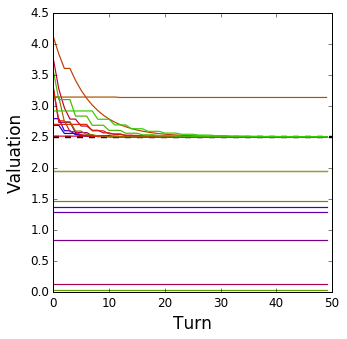
\includegraphics[width=7cm]{best1.png}
  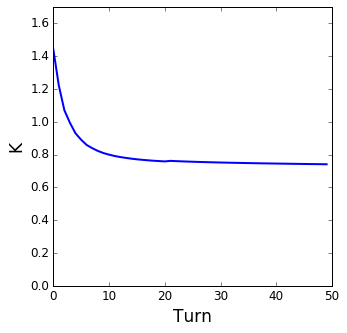
\includegraphics[width=6cm]{best2.png}
  \caption{Simulation with:  restaurant, persons, no friend, turns, best thinking choosing.}
\end{figure}
This situation may seems to be sensible if the restaurant is a really bad one, but would be ungodly if the restaurant is indeed a good one; in light of this, could happen that a good restaurant would be never discovered by someone just because the agent is convinced since the beginning (in real life, maybe because he heard about that) that the quality of it is really low.
However, this issue could be resolved through the introduction of the communication between friends


\section{Third simulation: a bit more complicated}
The simulations we considered until now are indeed too simple to reproduce a satisfying situation describing what happens in a real world; as a matter of fact, we could assume that people usually choose what they think is the best but we reasonably suppose that they will also explore the world. 
In this sense we introduce a bit more complex situation where we organize the probability of adopting a strategy instead of another in a different way: 50\% of time people goes to a restaurant randomly without considering its rank (random choose) and  remaining 50\% of time they go to the one they think is the best choice.
\begin{figure}[h]
  \centering
  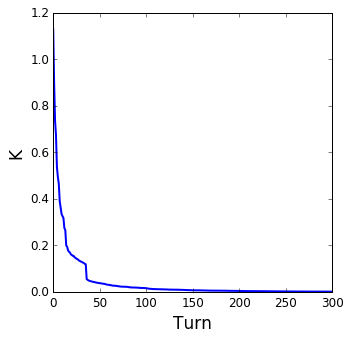
\includegraphics[width=7cm]{50501.png}
  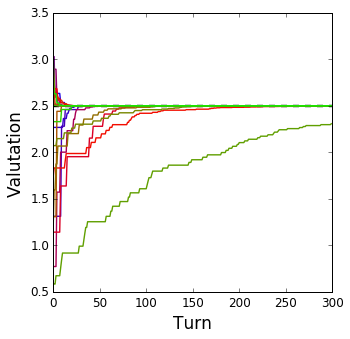
\includegraphics[width=6cm]{50502.png}
  \caption{Particular situation for a fixed restaurant. Simulation with: 4 restaurant, 20 persons, no friend, 300 turns, fifty-fifty.}
\end{figure}
Looking at the uncertainty factor $K_re$, introduced before, we observe that people are more incline in discovering new places even if they think, at first, they are not so good.
Moreover, in this case, we notice that people thought will converge to the real best restaurant, which rank is fixed to 2.5, faster than before and, furthermore, every person will convince itself that the best restaurant is indeed that one. 
This, simply means that more open-minded people, who are incline to try even places they don’t think are so good at first, will soon recognize which restaurant is the best one.



\section{Fourth simulation: communication among friends }
In this section we start to introduce the communication among people. Thus, a person can communicate its thought to another. 
People base the choice of the restaurant again on both two strategies: the 50\% of turns they will adopt random choose, remaining ones they will go for best  choose.
Due to how we set the parameters in this simulation we obtain a more stochastic one because of the random choice (the 50\% of the time) and even produced by the fact that people could easily find full a restaurant; as a matter of fact the capacity of each place is finite.
In this sense, we need to make many different simulations that represent a single realization of the model.


\subsection{Many friends means better choice}
In this subsection we deserved to study how the parameter $K$ changes in accord to the number of friends. We organize 4 different experiments incrementing the number of friends from 0 to 1,3 and 5 performing different realizations each.
In all experiment we set 20 people, 4 restaurants and 70 turns (time step conceived as 70 days).

Start considering the case with no friends. We plot $K(t)$ for all the 15 realizations of the experiment in  Fig:\ref{fig:15re}.
\begin{figure}[hbt]
  \centering
  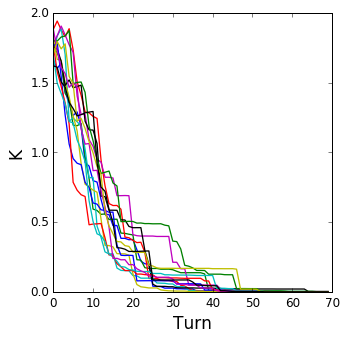
\includegraphics[width=9cm]{Koverall.png}
  \caption{}
  \label{fig:15re}
\end{figure}
Than we compute the mean and the variance of $K(t)$ over all this different realizations (green curve) and try to approximate it with an exponential (red curve), Fig:\ref{fig:aprox}.
\begin{figure}[hbt]
  \centering
  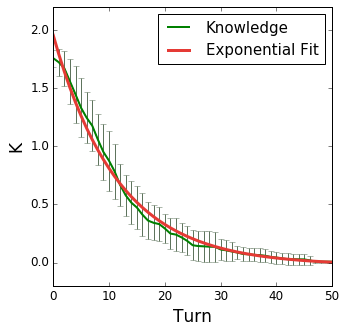
\includegraphics[width=9cm]{koverallMean.png}
  \label{fig:aprox}
  \caption{}
\end{figure} 
The exponential regression is good as confirm by a chi-square test.\\
$${\chi ^2} = 43.4 \text{ with } DF = 47$$
In particular the coefficients of the curve are:
\[K\left( t \right) = a{e^{ - bt + c}}\] 
\[\begin{array}{l}
a = 1.97\\
b = 0.086\\
c =  - 0.02
\end{array}\]
It can be interesting consider the exponential \textbf{time constant} $\tau  = \frac{1}{b} = 11.5$. This time constant can be interpretate as the number of turns needed to reduce $K$ by 63\% and approximately in $5 \tau = 57$ turns, the $K$ can be considered $0$, in other words after 57 turns the global uncertainty is zero.


We reproduce the same analysis done with no friends experiment for the other cases with the different number of friends.
Plotting the $K$ coefficient for all the different cases (Fig:\ref{fig:4curves}), we can see that model with higher number of friends have $K$ that go to zero faster then other (Table:\ref{tab:tabella}), this is the consequence of the fact that persons inform each other about the quality of restaurants and in less time discover the real rating.
\begin{figure}[b]
  \centering
  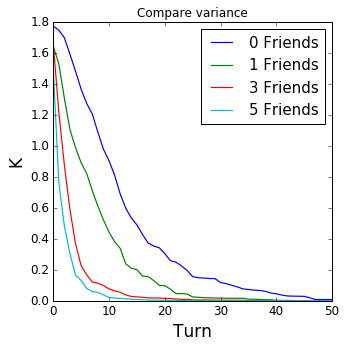
\includegraphics[width=9cm]{varAmici.png}
  \caption{}
  \label{fig:4curves}
\end{figure}

\begin{table}[b]
\centering
\caption{}
\label{tab:tabella}
\begin{tabular}{lccc}
\hline
\rowcolor[HTML]{C0C0C0} 
\multicolumn{1}{c}{\cellcolor[HTML]{C0C0C0}n friends} & $b$ coefficent                 & $\tau$                    & n turn to zero          \\ \hline
\multicolumn{1}{|l|}{{\color[HTML]{333333} 0}}        & \multicolumn{1}{c|}{- 0.086}   & \multicolumn{1}{c|}{11.5} & \multicolumn{1}{c|}{58} \\ \hline
\multicolumn{1}{|l|}{1}                               & \multicolumn{1}{c|}{- 0.134}   & \multicolumn{1}{c|}{7.4}  & \multicolumn{1}{c|}{37} \\ \hline
\multicolumn{1}{|l|}{3}                               & \multicolumn{1}{c|}{- 0.359}   & \multicolumn{1}{c|}{2.7}  & \multicolumn{1}{c|}{14} \\ \hline
\multicolumn{1}{|l|}{5}                               & \multicolumn{1}{c|}{- 0.560} & \multicolumn{1}{c|}{1.8}  & \multicolumn{1}{c|}{9}  \\ \hline
\end{tabular}
\end{table}














\end{document}
